% Name: Two-step reaction profile
% Description: A reaction that passes through an intermediate between two transition states; the first step has the larger barrier, so it limits the rate.
% Tags: reaction profile, intermediate, transition state, rate-determining step

\usetikzlibrary{arrows.meta}

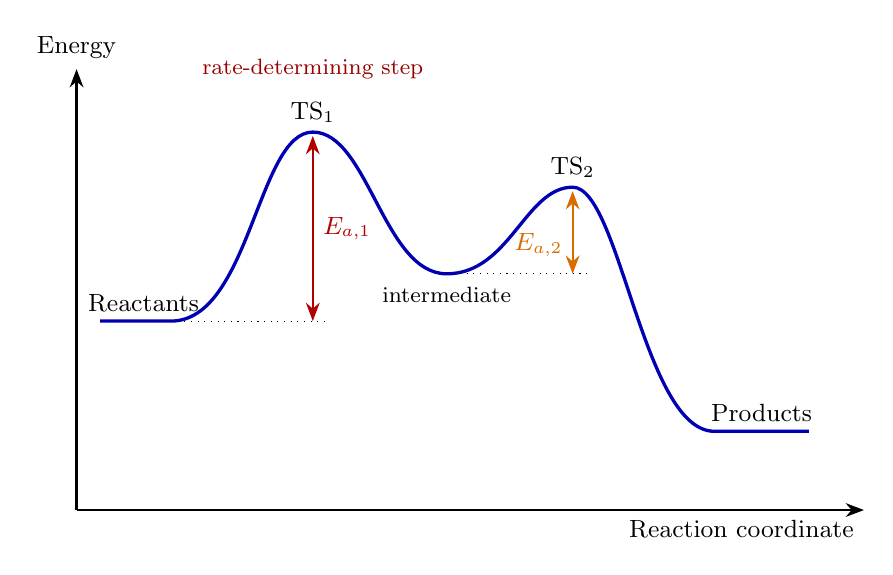
\begin{tikzpicture}[>={Stealth}, every node/.style={font=\small}]
  \draw[->, thick] (0,0) -- (10,0) node[below left] {Reaction coordinate};
  \draw[->, thick] (0,0) -- (0,5.6) node[above] {Energy};
  % Reactants 2.4, TS1 4.8, intermediate 3.0, TS2 4.1, products 1.0
  \draw[very thick, blue!70!black] (0.3,2.4) -- (1.2,2.4) .. controls (2.2,2.4) and (2.3,4.8) .. (3,4.8) .. controls (3.7,4.8) and (3.9,3) .. (4.7,3) .. controls (5.5,3) and (5.7,4.1) .. (6.3,4.1) .. controls (6.9,4.1) and (7.2,1) .. (8.1,1) -- (9.3,1);
  \node[above] at (0.85,2.4) {Reactants};
  \node[above] at (8.7,1) {Products};
  \node[above] at (3,4.8) {TS$_1$};
  \node[above] at (6.3,4.1) {TS$_2$};
  \node[below, align=center, font=\footnotesize] at (4.7,2.95) {intermediate};
  % Each barrier is measured straight down from its transition state to the level before it
  \draw[dotted] (1.2,2.4) -- (3.2,2.4) (4.7,3) -- (6.5,3);
  \draw[<->, thick, red!70!black] (3,2.4) -- node[right] {$E_{a,1}$} (3,4.75);
  \draw[<->, thick, orange!85!black] (6.3,3) -- node[left, pos=0.35] {$E_{a,2}$} (6.3,4.05);
  \node[font=\footnotesize, red!60!black, align=center] at (3,5.6) {rate-determining step};
\end{tikzpicture}
